% ----------------------------------
% Cap Captura de Requisitos
% ----------------------------------

\chapter{Captura de requisitos} % (fold)
\label{cha:captura_de_requisitos}
	
	En este apartado se describe de forma detallada cada una de las funcionalidades que pueden componer el proyecto, con el fin de guiar el desarrollo hacia el sistema correcto. El proceso estará apoyado en una lista de características y en el modelo del dominio.

% 
% Sec Lista de características
%
\section{Lista de características} % (fold)
	\label{sec:lista_de_caracteristicas}
	
	Cada característica tiene un nombre corto y una breve explicación, información suficiente para poder hablar de ella durante la planificación del producto. Cada característica tiene también un conjunto de valores de planificación que son incluidos:
	
	\begin{itemize}
		\item{Prioridad}
		\item{Estado}
		\item{Coste estimado de implementación}
		\item{Nivel de riesgo asociado a la implementación de la característica}
	\end{itemize}
	
%
% Sub Navegación (A)
%
\subsection{Navegación(A)} % (fold)
	\label{sub:lc_navegacion}
	
	\begin{center}
		\begin{tabularx}{15cm}{|X|}
			\hline 
				\bf{LC-A1. Tour de la aplicación}\\
			\hline
				Se debe mostrar una página estática como interfaz de entrada con un tour de las características de la aplicación, mostrando la potencia de la misma. Se incluyen páginas acerca de cada uno de los módulos que se gestionan y capturas de pantalla de las mismas.\\
			\hline
				\it{Prioridad}\\
			\hline
				\it{Estado}\\
			\hline
				\it{Coste}\\
			\hline
				\it{Riesgo}\\
			\hline
		\end{tabularx}
	\end{center}
	
	\begin{center}
		\begin{tabularx}{15cm}{|X|}
			\hline 
				\bf{LC-A2. Términos legales}\\
			\hline
				El sistema debe mostrar una página estática con los términos.\\
			\hline
				\it{Prioridad}\\
			\hline
				\it{Estado}\\
			\hline
				\it{Coste}\\
			\hline
				\it{Riesgo}\\
			\hline
		\end{tabularx}
	\end{center}
	
	\begin{center}
		\begin{tabularx}{15cm}{|X|}
			\hline 
				\bf{LC-A3. Condiciones de uso}\\
			\hline
				El sistema debe mostrar una página estática con las condiciones de uso y privacidad de información.\\
			\hline
				\it{Prioridad}\\
			\hline
				\it{Estado}\\
			\hline
				\it{Coste}\\
			\hline
				\it{Riesgo}\\
			\hline
		\end{tabularx}
	\end{center}
	
	\begin{center}
		\begin{tabularx}{15cm}{|X|}
			\hline 
				\bf{LC-A4. Referencias a la aplicación}\\
			\hline
				Se muestra una página estática con las referencias al producto realizadas por los entrenadores expertos que han participado en la elaboración de la aplicación.\\
			\hline
				\it{Prioridad}\\
			\hline
				\it{Estado}\\
			\hline
				\it{Coste}\\
			\hline
				\it{Riesgo}\\
			\hline
		\end{tabularx}
	\end{center}
	
	\begin{center}
		\begin{tabularx}{15cm}{|X|}
			\hline 
				\bf{LC-A5. Mostrar planes del producto}\\
			\hline
				Se muestra una página estática haciendo referencia a los diferentes planes de contratación del producto, especificando las características de las versiones gratuitas y de pago.\\
			\hline
				\it{Prioridad}\\
			\hline
				\it{Estado}\\
			\hline
				\it{Coste}\\
			\hline
				\it{Riesgo}\\
			\hline
		\end{tabularx}
	\end{center}		

	\begin{center}
		\begin{tabularx}{15cm}{|X|}
			\hline 
				\bf{LC-A6. Contactar con administrador de la aplicación}\\
			\hline
				Se debe incluir un formulario de contacto para que los usuarios puedan ponerse en contacto con los administradores del sitio.\\
			\hline
				\it{Prioridad}\\
			\hline
				\it{Estado}\\
			\hline
				\it{Coste}\\
			\hline
				\it{Riesgo}\\
			\hline
		\end{tabularx}
	\end{center}
	
	\begin{center}
		\begin{tabularx}{15cm}{|X|}
			\hline 
				\bf{LC-A7. Soporte para multilenguaje}\\
			\hline
				La aplicación se adaptará a distintos idiomas (español e inglés). Se adaptan los elementos de interfaz, siendo el idioma por defecto el español.\\
			\hline
				\it{Prioridad}\\
			\hline
				\it{Estado}\\
			\hline
				\it{Coste}\\
			\hline
				\it{Riesgo}\\
			\hline
		\end{tabularx}
	\end{center}
	
	\begin{center}
		\begin{tabularx}{15cm}{|X|}
			\hline 
				\bf{LC-A8. Compartir aplicación}\\
			\hline
				Los usuarios deben poder compartir la aplicación a través de enlaces facebook/twitter o enviando notificaciones por correo a contactos.\\
			\hline
				\it{Prioridad}\\
			\hline
				\it{Estado}\\
			\hline
				\it{Coste}\\
			\hline
				\it{Riesgo}\\
			\hline
		\end{tabularx}
	\end{center}
	
% subsection navegación_a_ (end)

% 
% Sub Gestión de entrenadores
%
\subsection{Gestión de entrenadores (B)} % (fold)
	\label{sub:gestion_de_entrenadores}
	
	\begin{center}
		\begin{tabularx}{15cm}{|X|}
			\hline 
				\bf{LC-B1. Registro en el sistema}\\
			\hline
				La aplicación debe permitir registrarse a los entrenadores en el sistema.\\
			\hline
				\it{Prioridad}\\
			\hline
				\it{Estado}\\
			\hline
				\it{Coste}\\
			\hline
				\it{Riesgo}\\
			\hline
		\end{tabularx}
	\end{center}
	
	\begin{center}
		\begin{tabularx}{15cm}{|X|}
			\hline 
				\bf{LC-B2. Acceso y autenticación}\\
			\hline
				Los entrenadores deben poder acceder al sistema, autenticándose con un nombre de usuario y contraseña. El sistema debe permitir recordar contraseña en caso de haberla olvidado.\\
			\hline
				\it{Prioridad}\\
			\hline
				\it{Estado}\\
			\hline
				\it{Coste}\\
			\hline
				\it{Riesgo}\\
			\hline
		\end{tabularx}
	\end{center}

	\begin{center}
		\begin{tabularx}{15cm}{|X|}
			\hline 
				\bf{LC-B3. Acceso con cuenta de facebook o twitter}\\
			\hline
				El sistema puede permitir el acceso al sistema usando cuenta de facebook o twitter, integrando así la información proporcionada en las redes sociales.\\
			\hline
				\it{Prioridad}\\
			\hline
				\it{Estado}\\
			\hline
				\it{Coste}\\
			\hline
				\it{Riesgo}\\
			\hline
		\end{tabularx}
	\end{center}
	
	\begin{center}
		\begin{tabularx}{15cm}{|X|}
			\hline 
				\bf{LC-B4. Cerrar sesión}\\
			\hline
				Los entrenadores podrán cerrar la sesión iniciada cuando se finalicen las tareas de gestión deportiva de su equipo.\\
			\hline
				\it{Prioridad}\\
			\hline
				\it{Estado}\\
			\hline
				\it{Coste}\\
			\hline
				\it{Riesgo}\\
			\hline
		\end{tabularx}
	\end{center}
	
	\begin{center}
		\begin{tabularx}{15cm}{|X|}
			\hline 
				\bf{LC-B5. Mostrar ayuda del registro y autenticación}\\
			\hline
				El sistema debe mostrar ayuda referente al proceso de registro y autenticación de los entrenadores en el sistema.\\
			\hline
				\it{Prioridad}\\
			\hline
				\it{Estado}\\
			\hline
				\it{Coste}\\
			\hline
				\it{Riesgo}\\
			\hline
		\end{tabularx}
	\end{center}
	
	\begin{center}
		\begin{tabularx}{15cm}{|X|}
			\hline 
				\bf{LC-B6. Acceso al dashboard}\\
			\hline
				El sistema debe permitir a los entrenadores ir a la página \it{dashboard} (resumen). En ella se muestran las opciones más usadas en el proceso, así como una pantalla resumen para comenzar a usar la aplicación: terminar de configurar los datos, añadir los primeros nadadores, crear entrenamientos/test/competiciones e invitar contactos a la aplicación.\\
			\hline
				\it{Prioridad}\\
			\hline
				\it{Estado}\\
			\hline
				\it{Coste}\\
			\hline
				\it{Riesgo}\\
			\hline
		\end{tabularx}
	\end{center}
	
	\begin{center}
		\begin{tabularx}{15cm}{|X|}
			\hline 
				\bf{LC-B7. Configuración del perfil}\\
			\hline
				Los entrenadores que accedan al sistema pueden modificar su perfil. Se trata de modificar datos insertados en el registro, tanto de información personal como datos de contacto.\\
			\hline
				\it{Prioridad}\\
			\hline
				\it{Estado}\\
			\hline
				\it{Coste}\\
			\hline
				\it{Riesgo}\\
			\hline
		\end{tabularx}
	\end{center}
	
	\begin{center}
		\begin{tabularx}{15cm}{|X|}
			\hline 
				\bf{LC-B8. Recibir notificaciones por email}\\
			\hline
				Los entrenadores pueden comunicar en su perfil que desean recibir notificaciones de actualizaciones a través del email.\\
			\hline
				\it{Prioridad}\\
			\hline
				\it{Estado}\\
			\hline
				\it{Coste}\\
			\hline
				\it{Riesgo}\\
			\hline
		\end{tabularx}
	\end{center}
	
	\begin{center}
		\begin{tabularx}{15cm}{|X|}
			\hline 
				\bf{LC-B9. Configurar apariencia para informes}\\
			\hline
				Los entrenadores pueden modificar la apariencia de los informes que se generen. Lo principal es añadir un logo del equipo en el que trabaja, para posteriormente mostrarlo en la cabecera del informe.\\
			\hline
				\it{Prioridad}\\
			\hline
				\it{Estado}\\
			\hline
				\it{Coste}\\
			\hline
				\it{Riesgo}\\
			\hline
		\end{tabularx}
	\end{center}
	
	\begin{center}
		\begin{tabularx}{15cm}{|X|}
			\hline 
				\bf{LC-B10. Contratar plan \it{premium}}\\
			\hline
				Los entrenadores deben poder contratar los planes premium que se definan para la aplicación. Contienen funcionalidades extras definidas. El pago del plan tiene que ser a través de plataforma \it{paypal}\\
			\hline
				\it{Prioridad}\\
			\hline
				\it{Estado}\\
			\hline
				\it{Coste}\\
			\hline
				\it{Riesgo}\\
			\hline
		\end{tabularx}
	\end{center}
	
	\begin{center}
		\begin{tabularx}{15cm}{|X|}
			\hline 
				\bf{LC-B11. Configurar índice Mujika}\\
			\hline
				Los entrenadores deben poder modificar el índice de Mujika, el cuál es un parámetro que define el factor de multiplicación del volumen para obtener la carga de un entrenamiento. Será usado para calcular los datos estadísticos de los entrenamientos.\\
			\hline
				\it{Prioridad}\\
			\hline
				\it{Estado}\\
			\hline
				\it{Coste}\\
			\hline
				\it{Riesgo}\\
			\hline
		\end{tabularx}
	\end{center}
	
	\begin{center}
		\begin{tabularx}{15cm}{|X|}
			\hline 
				\bf{LC-B12. Lista de contactos entrenadores}\\
			\hline
				Los entrenadores puede añadir/eliminar listas de contactos, donde aparecen otros entrenadores que están registrados en la aplicación. Cada lista es personal, pudiendo exportar los contactos a Excel o CSV.\\
			\hline
				\it{Prioridad}\\
			\hline
				\it{Estado}\\
			\hline
				\it{Coste}\\
			\hline
				\it{Riesgo}\\
			\hline
		\end{tabularx}
	\end{center}
	
	\begin{center}
		\begin{tabularx}{15cm}{|X|}
			\hline 
				\bf{LC-B13. Mensajería entre entrenadores}\\
			\hline
				El sistema debe permitir el envío de mensajes privados entre entrenadores que están registrados en la aplicación. La lista de contactos es la base para poder realizar el contacto con otros entrenadores.\\
			\hline
				\it{Prioridad}\\
			\hline
				\it{Estado}\\
			\hline
				\it{Coste}\\
			\hline
				\it{Riesgo}\\
			\hline
		\end{tabularx}
	\end{center}
% subsection gestión_de_entrenadores_b_ (end)

%
% Sub Gestión de diario del entrenador
%
\subsection{Gestión de diario del entrenador (C)} % (fold)
	\label{sub:gestion_diario_entrenador}

	\begin{center}
		\begin{tabularx}{15cm}{|X|}
			\hline 
				\bf{LC-C1. Ver diario}\\
			\hline
				El sistema debe permitir a los entrenadores ver el contenido del diario. En él se muestran todos los registros insertados por el entrenador, mostrando título y fecha de creación. Desde ahí se puede acceder a cada uno de los registros para ver el contenido de los mismos.\\
			\hline
				\it{Prioridad}\\
			\hline
				\it{Estado}\\
			\hline
				\it{Coste}\\
			\hline
				\it{Riesgo}\\
			\hline
		\end{tabularx}
	\end{center}
	
	\begin{center}
		\begin{tabularx}{15cm}{|X|}
			\hline 
				\bf{LC-C2. Añadir/Eliminar/Modificar registro en el diario}\\
			\hline
				El entrenador puede añadir, eliminar o modificar registros en su diario. Cada registro muestra una incidencia u observación que quiere reflejar el entrenador.\\
			\hline
				\it{Prioridad}\\
			\hline
				\it{Estado}\\
			\hline
				\it{Coste}\\
			\hline
				\it{Riesgo}\\
			\hline
		\end{tabularx}
	\end{center}
	
	\begin{center}
		\begin{tabularx}{15cm}{|X|}
			\hline 
				\bf{LC-C3. Añadir etiqueta a un registro del diario}\\
			\hline
				El sistema debe permitir que un entrenador añada etiquetas a cada uno de los registros del diario. Esto permite agrupar incidencias u observaciones por temática, con lo que ayudaría al entrenador a localizarlas más fácilmente.\\
			\hline
				\it{Prioridad}\\
			\hline
				\it{Estado}\\
			\hline
				\it{Coste}\\
			\hline
				\it{Riesgo}\\
			\hline
		\end{tabularx}
	\end{center}
	
	\begin{center}
		\begin{tabularx}{15cm}{|X|}
			\hline 
				\bf{LC-C4. Buscar un registro en el diario}\\
			\hline
				El sistema debe permitir que los entrenadores busquen registros en sus diarios. Las búsquedas pueden ser por fechas, títulos o etiquetas asociadas.\\
			\hline
				\it{Prioridad}\\
			\hline
				\it{Estado}\\
			\hline
				\it{Coste}\\
			\hline
				\it{Riesgo}\\
			\hline
		\end{tabularx}
	\end{center}
	
	\begin{center}
		\begin{tabularx}{15cm}{|X|}
			\hline 
				\bf{LC-C5. Resumen del diario}\\
			\hline
				La aplicación debe mostrar en la página ``Ver diario'' un resumen con la cantidad de registros insertados en el diario y las etiquetas más usadas.\\
			\hline
				\it{Prioridad}\\
			\hline
				\it{Estado}\\
			\hline
				\it{Coste}\\
			\hline
				\it{Riesgo}\\
			\hline
		\end{tabularx}
	\end{center}
	
	\begin{center}
		\begin{tabularx}{15cm}{|X|}
			\hline 
				\bf{LC-C6. Adjuntar fichero en un registro del diario}\\
			\hline
				Los entrenadores deben poder adjuntar ficheros en un registro del diario. Estos ficheros podrán ser descargados y abiertos por los entrenadores posteriormente.\\
			\hline
				\it{Prioridad}\\
			\hline
				\it{Estado}\\
			\hline
				\it{Coste}\\
			\hline
				\it{Riesgo}\\
			\hline
		\end{tabularx}
	\end{center}
	
	\begin{center}
		\begin{tabularx}{15cm}{|X|}
			\hline 
				\bf{LC-C7. Imprimir diario}\\
			\hline
				El sistema debe permitir que el entrenador imprima todo el diario completo. Se muestra la fecha de creación, título y contenido de cada registro insertado en el diario. Así mismo, también debe permitir el imprimir únicamente un registro determinado.\\
			\hline
				\it{Prioridad}\\
			\hline
				\it{Estado}\\
			\hline
				\it{Coste}\\
			\hline
				\it{Riesgo}\\
			\hline
		\end{tabularx}
	\end{center}

% subsection gestión_de_diario_del_entrenador_c_ (end)

% 
% Sub Gestión de nadadores
%
\subsection{Gestión de nadadores (D)} % (fold)
	\label{sub:gestion_de_nadadores}
	
	\begin{center}
		\begin{tabularx}{15cm}{|X|}
			\hline 
				\bf{LC-D1. Ver nadadores}\\
			\hline
				El sistema debe permitir al entrenador ver el listado de nadadores insertados. Listado con los datos más usados para localizar lo más rápido posible a los nadadores. Sirve de interfaz para ver las fichas individuales de los nadadores.\\
			\hline
				\it{Prioridad}\\
			\hline
				\it{Estado}\\
			\hline
				\it{Coste}\\
			\hline
				\it{Riesgo}\\
			\hline
		\end{tabularx}
	\end{center}
	
	\begin{center}
		\begin{tabularx}{15cm}{|X|}
			\hline 
				\bf{LC-D2. Añadir/Eliminar/Modificar nadador}\\
			\hline
				El entrenador debe poder añadir, eliminar o modificar un nadador. Cada ficha del nadador tendrá asociado unos datos personales e información generada al introducir datos en las competiciones y test.\\
			\hline
				\it{Prioridad}\\
			\hline
				\it{Estado}\\
			\hline
				\it{Coste}\\
			\hline
				\it{Riesgo}\\
			\hline
		\end{tabularx}
	\end{center}
	
	\begin{center}
		\begin{tabularx}{15cm}{|X|}
			\hline 
				\bf{LC-D3. Añadir fotografía}\\
			\hline
				El entrenador debe poder insertar una fotografía del nadador, la cuál se almacenará en el sistema y se mostrará en el perfil.\\
			\hline
				\it{Prioridad}\\
			\hline
				\it{Estado}\\
			\hline
				\it{Coste}\\
			\hline
				\it{Riesgo}\\
			\hline
		\end{tabularx}
	\end{center}
	
	\begin{center}
		\begin{tabularx}{15cm}{|X|}
			\hline 
				\bf{LC-D4. Exportar nadadores a Excel}\\
			\hline
				Los entrenadores pueden enviar a una hoja Excel el listado de nadadores que contiene. Sólo se exportan los datos personales.\\
			\hline
				\it{Prioridad}\\
			\hline
				\it{Estado}\\
			\hline
				\it{Coste}\\
			\hline
				\it{Riesgo}\\
			\hline
		\end{tabularx}
	\end{center}
	
	\begin{center}
		\begin{tabularx}{15cm}{|X|}
			\hline 
				\bf{LC-D5. Imprimir lista de nadadores}\\
			\hline
				El sistema debe permitir al entrenador imprimir el listado de todos los nadadores pertenecientes al entrenador, así como las fichas individuales de cada nadador. En el caso de imprimir fichas individuales, se debe imprimir la información referente a cada prueba de las competiciones y a los test.\\
			\hline
				\it{Prioridad}\\
			\hline
				\it{Estado}\\
			\hline
				\it{Coste}\\
			\hline
				\it{Riesgo}\\
			\hline
		\end{tabularx}
	\end{center}
	
	\begin{center}
		\begin{tabularx}{15cm}{|X|}
			\hline 
				\bf{LC-D6. Enviar lista de nadadores por email}\\
			\hline
				El sistema debe permitir al entrenador enviar por email el listado de todos los nadadores pertenecientes al entrenador, así como las fichas individuales de cada nadador.\\
			\hline
				\it{Prioridad}\\
			\hline
				\it{Estado}\\
			\hline
				\it{Coste}\\
			\hline
				\it{Riesgo}\\
			\hline
		\end{tabularx}
	\end{center}
	
	\begin{center}
		\begin{tabularx}{15cm}{|X|}
			\hline 
				\bf{LC-D7. Contactar con nadadores vía email}\\
			\hline
				El entrenador debe poder enviar email a los nadadores. En caso de ser menores de edad, la dirección de contacto debe ser la de los padres. Puede ser un contacto individual o colectivo.\\
			\hline
				\it{Prioridad}\\
			\hline
				\it{Estado}\\
			\hline
				\it{Coste}\\
			\hline
				\it{Riesgo}\\
			\hline
		\end{tabularx}
	\end{center}
	
	\begin{center}
		\begin{tabularx}{15cm}{|X|}
			\hline 
				\bf{LC-D8. Estadísticas de los nadadores}\\
			\hline
				El sistema debe generar estadísticas acerca de los nadadores. Están relacionadas con el número de nadadores dados de alta en un mismo mes; gráfico para ver la mejora de las marcas individuales de cada nadador; gráfico para ver la mejora en los test realizados.\\
			\hline
				\it{Prioridad}\\
			\hline
				\it{Estado}\\
			\hline
				\it{Coste}\\
			\hline
				\it{Riesgo}\\
			\hline
		\end{tabularx}
	\end{center}
	
	\begin{center}
		\begin{tabularx}{15cm}{|X|}
			\hline 
				\bf{LC-D9. Cálculo de \%MM de cada nadador}\\
			\hline
				El sistema debe calcular los valores de porcentaje respecto a la mejor marca de un nadador. Por ejemplo: 80\% respecto a la mejor marca.\\
			\hline
				\it{Prioridad}\\
			\hline
				\it{Estado}\\
			\hline
				\it{Coste}\\
			\hline
				\it{Riesgo}\\
			\hline
		\end{tabularx}
	\end{center}
	
	\begin{center}
		\begin{tabularx}{15cm}{|X|}
			\hline 
				\bf{LC-D10. Búsqueda de nadadores}\\
			\hline
				El entrenador debe poder hacer búsquedas sobre los nadadores. Los principales filtros son los nombres y las categorías del nadador.\\
			\hline
				\it{Prioridad}\\
			\hline
				\it{Estado}\\
			\hline
				\it{Coste}\\
			\hline
				\it{Riesgo}\\
			\hline
		\end{tabularx}
	\end{center}
	
% subsection gestión_de_nadadores_d_ (end)

%
% Sub Gestión de entrenamientos
%
\subsection{Gestión de entrenamientos (E)} % (fold)
	\label{sub:gestion_de_entrenamientos}

	\begin{center}
		\begin{tabularx}{15cm}{|X|}
			\hline 
				\bf{LC-E1. Añadir planificación}\\
			\hline
				El entrenador debe poder crear una hoja de cálculo con la planificación de la temporada. Se tienen en cuenta los volúmenes y cargas de los entrenamientos.\\
			\hline
				\it{Prioridad}\\
			\hline
				\it{Estado}\\
			\hline
				\it{Coste}\\
			\hline
				\it{Riesgo}\\
			\hline
		\end{tabularx}
	\end{center}
	
	\begin{center}
		\begin{tabularx}{15cm}{|X|}
			\hline 
				\bf{LC-E2. Subir planificación}\\
			\hline
				El entrenador debe poder subir al sistema un fichero Excel o pdf con la planificación de la temporada. Este fichero servirá para comparar el volumen y carga de los microciclos \footnote{Estructura de organización del entrenamiento que están constituidos por las sesiones de entrenamientos.} y macrociclos \footnote{Estructura de organización del entrenamiento que están constituidos por un conjunto de microciclos.}\\
			\hline
				\it{Prioridad}\\
			\hline
				\it{Estado}\\
			\hline
				\it{Coste}\\
			\hline
				\it{Riesgo}\\
			\hline
		\end{tabularx}
	\end{center}
	
	\begin{center}
		\begin{tabularx}{15cm}{|X|}
			\hline 
				\bf{LC-E3. Imprimir planificación}\\
			\hline
				El sistema debe permitir al entrenador imprimir la planificación de la temporada, tanto en caso de que se haya creado en el sistema como si se ha subido a la aplicación.\\
			\hline
				\it{Prioridad}\\
			\hline
				\it{Estado}\\
			\hline
				\it{Coste}\\
			\hline
				\it{Riesgo}\\
			\hline
		\end{tabularx}
	\end{center}
	
	\begin{center}
		\begin{tabularx}{15cm}{|X|}
			\hline 
				\bf{LC-E4. Ver entrenamientos}\\
			\hline
				El sistema debe permitir al entrenador ver el listado de entrenamientos insertados. Cada sesión incluye los ejercicios que se realizan en un entrenamiento diario. Puede usarse un calendario para verlo más fácilmente.\\
			\hline
				\it{Prioridad}\\
			\hline
				\it{Estado}\\
			\hline
				\it{Coste}\\
			\hline
				\it{Riesgo}\\
			\hline
		\end{tabularx}
	\end{center}
	
	\begin{center}
		\begin{tabularx}{15cm}{|X|}
			\hline 
				\bf{LC-E5. Añadir/Modificar/Eliminar entrenamiento}\\
			\hline
				El sistema debe permitir al entrenador añadir, modificar o eliminar entrenamientos. Cada entrenamiento consta de una serie de ejercicios que lo forman y representa una sesión de entrenamiento.\\
			\hline
				\it{Prioridad}\\
			\hline
				\it{Estado}\\
			\hline
				\it{Coste}\\
			\hline
				\it{Riesgo}\\
			\hline
		\end{tabularx}
	\end{center}
	
	\begin{center}
		\begin{tabularx}{15cm}{|X|}
			\hline 
				\bf{LC-E6. Añadir ejercicio al entrenamiento}\\
			\hline
				El entrenador debe poder introducir ejercicios en cada uno de los entrenamientos. Cada ejercicio es de un tipo específico.\\
			\hline
				\it{Prioridad}\\
			\hline
				\it{Estado}\\
			\hline
				\it{Coste}\\
			\hline
				\it{Riesgo}\\
			\hline
		\end{tabularx}
	\end{center}
	
	\begin{center}
		\begin{tabularx}{15cm}{|X|}
			\hline 
				\bf{LC-E7. Exportar entrenamiento a Excel}\\
			\hline
				El sistema debe permitir exportar una sesión de entrenamiento a Excel.\\
			\hline
				\it{Prioridad}\\
			\hline
				\it{Estado}\\
			\hline
				\it{Coste}\\
			\hline
				\it{Riesgo}\\
			\hline
		\end{tabularx}
	\end{center}
	
	\begin{center}
		\begin{tabularx}{15cm}{|X|}
			\hline 
				\bf{LC-E8. Imprimir entrenamientos}\\
			\hline
				El entrenador debe poder imprimir sesiones de entrenamientos. Puede seleccionarse un intervalo de sesiones de entrenamientos para proporcionar más usabilidad \footnote{Según ISO/IEC 9126, la usabilidad se refiere a la capacidad de un software de ser comprendido, aprendido, usado y ser atractivo para el usuario, en condiciones específicas de uso.}.\\
			\hline
				\it{Prioridad}\\
			\hline
				\it{Estado}\\
			\hline
				\it{Coste}\\
			\hline
				\it{Riesgo}\\
			\hline
		\end{tabularx}
	\end{center}
	
	\begin{center}
		\begin{tabularx}{15cm}{|X|}
			\hline 
				\bf{LC-E9. Enviar por mail entrenamiento }\\
			\hline
				El entrenador debe poder enviar por email una sesión de entrenamiento a un destinatario introducido.\\
			\hline
				\it{Prioridad}\\
			\hline
				\it{Estado}\\
			\hline
				\it{Coste}\\
			\hline
				\it{Riesgo}\\
			\hline
		\end{tabularx}
	\end{center}
	
	\begin{center}
		\begin{tabularx}{15cm}{|X|}
			\hline 
				\bf{LC-E10. Estadísticas de los entrenamientos}\\
			\hline
				El sistema debe generar estadísticas sobre los entrenamientos. Son referidas al volumen y carga de cada sesión de entrenamiento --- microciclo; al volumen y carga de cada macrociclo; volumen y carga de cada tipo de ejercicio. Estas estadísticas servirán parar compararlas con los datos de la planificación.\\
			\hline
				\it{Prioridad}\\
			\hline
				\it{Estado}\\
			\hline
				\it{Coste}\\
			\hline
				\it{Riesgo}\\
			\hline
		\end{tabularx}
	\end{center}
	
	\begin{center}
		\begin{tabularx}{15cm}{|X|}
			\hline 
				\bf{LC-E11. Búsqueda de un entrenamiento}\\
			\hline
				El entrenador debe poder buscar entre los entrenamientos insertados en la aplicación.\\
			\hline
				\it{Prioridad}\\
			\hline
				\it{Estado}\\
			\hline
				\it{Coste}\\
			\hline
				\it{Riesgo}\\
			\hline
		\end{tabularx}
	\end{center}
	
	\begin{center}
		\begin{tabularx}{15cm}{|X|}
			\hline 
				\bf{LC-E12. Cálculo del tiempo de un entrenamiento}\\
			\hline
				El sistema debe poder calcular el tiempo en que se tarda en realizar un entrenamiento con los ejercicios insertados. Se tiene que basar en un tiempo medio de los nadadores y en la intensidad en que se realizan los ejercicios.\\
			\hline
				\it{Prioridad}\\
			\hline
				\it{Estado}\\
			\hline
				\it{Coste}\\
			\hline
				\it{Riesgo}\\
			\hline
		\end{tabularx}
	\end{center}
% subsection gestión_de_entrenamientos_e_ (end)

%
% Sub Gestión de Competiciones
%
\subsection{Gestión de competiciones (F)} % (fold)
	\label{sub:gestion_de_competiciones}

	\begin{center}
		\begin{tabularx}{15cm}{|X|}
			\hline 
				\bf{LC-F1. Ver competiciones}\\
			\hline
				Los entrenadores deben poder ver un listado con todas las competiciones que han insertado en el sistema. Están organizadas por fecha, siendo las más recientes primero.\\
			\hline
				\it{Prioridad}\\
			\hline
				\it{Estado}\\
			\hline
				\it{Coste}\\
			\hline
				\it{Riesgo}\\
			\hline
		\end{tabularx}
	\end{center}
	
	\begin{center}
		\begin{tabularx}{15cm}{|X|}
			\hline 
				\bf{LC-F2. Añadir/Modificar/Eliminar competición }\\
			\hline
				Un entrenador debe poder añadir, modificar o eliminar una competición a la aplicación. Cada competición indica el lugar, la fecha, la piscina, el tipo de cronometraje y el tipo de piscina. Se almacenan los resultados de cada nadador en la competición.\\
			\hline
				\it{Prioridad}\\
			\hline
				\it{Estado}\\
			\hline
				\it{Coste}\\
			\hline
				\it{Riesgo}\\
			\hline
		\end{tabularx}
	\end{center}
	
	\begin{center}
		\begin{tabularx}{15cm}{|X|}
			\hline 
				\bf{LC-F3. Añadir resultado de un nadador }\\
			\hline
				El sistema debe permitir al entrenador insertar un resultado de un nadador en la competición. Este resultado se mostrará en la competición y en la ficha del nadador asociado.\\
			\hline
				\it{Prioridad}\\
			\hline
				\it{Estado}\\
			\hline
				\it{Coste}\\
			\hline
				\it{Riesgo}\\
			\hline
		\end{tabularx}
	\end{center}
	
	\begin{center}
		\begin{tabularx}{15cm}{|X|}
			\hline 
				\bf{LC-F4. Ver calendario}\\
			\hline
				El entrenador debe poder ver un calendario con las competiciones. Cada competición añadida al calendario se convertiría en un registro de la lista de competiciones.\\
			\hline
				\it{Prioridad}\\
			\hline
				\it{Estado}\\
			\hline
				\it{Coste}\\
			\hline
				\it{Riesgo}\\
			\hline
		\end{tabularx}
	\end{center}
	
	\begin{center}
		\begin{tabularx}{15cm}{|X|}
			\hline 
				\bf{LC-F5. Imprimir listado de competiciones}\\
			\hline
				El sistema debe permitir a los entrenadores imprimir el listado de las competiciones, así como la ficha de una competición individual. En las competiciones individuales se mostrarán los resultados de cada nadador en ella.\\
			\hline
				\it{Prioridad}\\
			\hline
				\it{Estado}\\
			\hline
				\it{Coste}\\
			\hline
				\it{Riesgo}\\
			\hline
		\end{tabularx}
	\end{center}
	
	\begin{center}
		\begin{tabularx}{15cm}{|X|}
			\hline 
				\bf{LC-F6. Añadir etiqueta a competición}\\
			\hline
				Los entrenadores deben poder añadir etiquetas a las competiciones, con el fin de catalogarlas y gestionarlas mejor.\\
			\hline
				\it{Prioridad}\\
			\hline
				\it{Estado}\\
			\hline
				\it{Coste}\\
			\hline
				\it{Riesgo}\\
			\hline
		\end{tabularx}
	\end{center}
	
	\begin{center}
		\begin{tabularx}{15cm}{|X|}
			\hline 
				\bf{LC-F7. Buscar competición}\\
			\hline
				El sistema debe permitir al entrenador buscar competiciones por nombre, fecha, piscina o etiqueta\\
			\hline
				\it{Prioridad}\\
			\hline
				\it{Estado}\\
			\hline
				\it{Coste}\\
			\hline
				\it{Riesgo}\\
			\hline
		\end{tabularx}
	\end{center}
	
	\begin{center}
		\begin{tabularx}{15cm}{|X|}
			\hline 
				\bf{LC-F8. Enviar por email competición}\\
			\hline
				El sistema debe permitir enviar los resultados de una competición por email.\\
			\hline
				\it{Prioridad}\\
			\hline
				\it{Estado}\\
			\hline
				\it{Coste}\\
			\hline
				\it{Riesgo}\\
			\hline
		\end{tabularx}
	\end{center}
	
	\begin{center}
		\begin{tabularx}{15cm}{|X|}
			\hline 
				\bf{LC-F9. Organizar competiciones}\\
			\hline
				El sistema debe permitir al entrenador organizar las listas de competiciones en orden ascendente y descendente.\\
			\hline
				\it{Prioridad}\\
			\hline
				\it{Estado}\\
			\hline
				\it{Coste}\\
			\hline
				\it{Riesgo}\\
			\hline
		\end{tabularx}
	\end{center}
	
% subsection gestión_de_competiciones_f_ (end)

%
% Sub Gestión de Test
%
\subsection{Gestión de Test (G)} % (fold)
	\label{sub:gestion_de_test}

	\begin{center}
		\begin{tabularx}{15cm}{|X|}
			\hline 
				\bf{LC-G1. Ver test}\\
			\hline
				El sistema debe permitir a los entrenadores ver el listado de test insertados en el sistema. Cada test representa un listado de pruebas realizadas sobre los nadadores.\\
			\hline
				\it{Prioridad}\\
			\hline
				\it{Estado}\\
			\hline
				\it{Coste}\\
			\hline
				\it{Riesgo}\\
			\hline
		\end{tabularx}
	\end{center}
	
	\begin{center}
		\begin{tabularx}{15cm}{|X|}
			\hline 
				\bf{LC-G2. Añadir/Modificar/Eliminar test}\\
			\hline
				El entrenador debe poder añadir, modificar o eliminar test al sistema. Dentro de cada test se incluyen los resultados de cada nadador. Debe existir una opción para poder añadir todos los nadadores de una determinada categoría, y posteriormente modificar el resultado del test. Cada resultado del test se añade al perfil del nadador relacionado.\\
			\hline
				\it{Prioridad}\\
			\hline
				\it{Estado}\\
			\hline
				\it{Coste}\\
			\hline
				\it{Riesgo}\\
			\hline
		\end{tabularx}
	\end{center}
	
	\begin{center}
		\begin{tabularx}{15cm}{|X|}
			\hline 
				\bf{LC-G3. Imprimir test}\\
			\hline
				El sistema debe permitir al entrenador imprimir el listado de test realizados. Así mismo, se debe dar la opción de imprimir cada test individualmente.\\
			\hline
				\it{Prioridad}\\
			\hline
				\it{Estado}\\
			\hline
				\it{Coste}\\
			\hline
				\it{Riesgo}\\
			\hline
		\end{tabularx}
	\end{center}
	
	\begin{center}
		\begin{tabularx}{15cm}{|X|}
			\hline 
				\bf{LC-G4. Enviar por email test}\\
			\hline
				El sistema debe permitir al entrenador enviar el listado de los test por email.\\
			\hline
				\it{Prioridad}\\
			\hline
				\it{Estado}\\
			\hline
				\it{Coste}\\
			\hline
				\it{Riesgo}\\
			\hline
		\end{tabularx}
	\end{center}
	\bigskip % Salto de línea grande
% subsection gestión_de_test_g_ (end)
% section lista_de_características (end)

%
%	Sec Modelo del dominio
%
\section{Modelo del dominio} % (fold)
	\label{sec:modelo_del_dominio}

%
% Sub Introducción
%
\subsection{Introducción} % (fold)
	\label{sub:md_introduccion}
	
	Un modelo del dominio (también conocido como modelo conceptual) explica los conceptos significativos en un dominio del problema; es el artefacto más importante a crear durante el análisis orientado a objetos \footnote{Los caos de uso son un importante artefacto del análisis de requerimientos, pero realmente no están orientados a {\it objetos}. Ponen de relieve la vista del dominio a partir de un proceso.}. 
	
	Un {\bf modelo del dominio} es una representación de conceptos en un dominio del problema\cite{Fowler96}\cite{MO95}. En UML, se ilustra con un grupo de {\bf diagramas de estructura estática} donde no se define ninguna operación. La designación de {\it modelo conceptual} ofrece la ventaja de subrayar fuertemente una concentración en los conceptos del dominio, no en las entidades del software.
	
	Puede mostrarnos:
	\begin{itemize}
		\item{conceptos}
		\item{asociaciones entre conceptos}
		\item{atributos de conceptos}
	\end{itemize}
	
	En términos informales el concepto es una idea, cosa u objeto. En un lenguaje más formal podemos considerarlo a partir de un símbolo, intensión \footnote{Intensión: en oposición a extensión, designa el grado de una cualidad.} y extensión \cite{MO95}.
	
	\begin{itemize}
		\item{{\bf Símbolo:} palabras o imágenes que representan un concepto.}
		\item{{\bf Intensión:} la definición del concepto.}
		\item{{\bf Extensión:} el conjunto de ejemplos a que se aplica el concepto.}
	\end{itemize}
	
	Los problemas de software a veces son complejos; la descomposición ---divide y vencerás--- es una estrategia que suele utilizarse para resolver la complejidad dividiendo el espacio del problema en unidades comprensibles. En el análisis orientado a objetos la dimensión de la descomposición se lleva a cabo fundamentalmente con conceptos.
		
	Por tanto, una tarea primordial de la fase de análisis consiste en identificar varios conceptos en el dominio y documentar los resultados en un modelo conceptual. Una cualidad que debe ofrecer un modelo conceptual es que representa cosas del mundo real, no componentes del software.
	
% subsection introducción (end)			

%
% Sub Contrucción del modelo del dominio
%
\subsection{Construcción del modelo del dominio} % (fold)
	\label{sub:construccion_del_modelo_del_dominio}

	El entrenador es la principal figura en el desarrollo deportivo de un equipo de natación, el cual es la persona que se encarga de un grupo de nadadores con el fin de obtener unos resultados a final de temporada. El proceso completo está definido en la figura \ref{fig:modelo_dominio}.
	
	 
	\begin{figure}
	  \centering
	    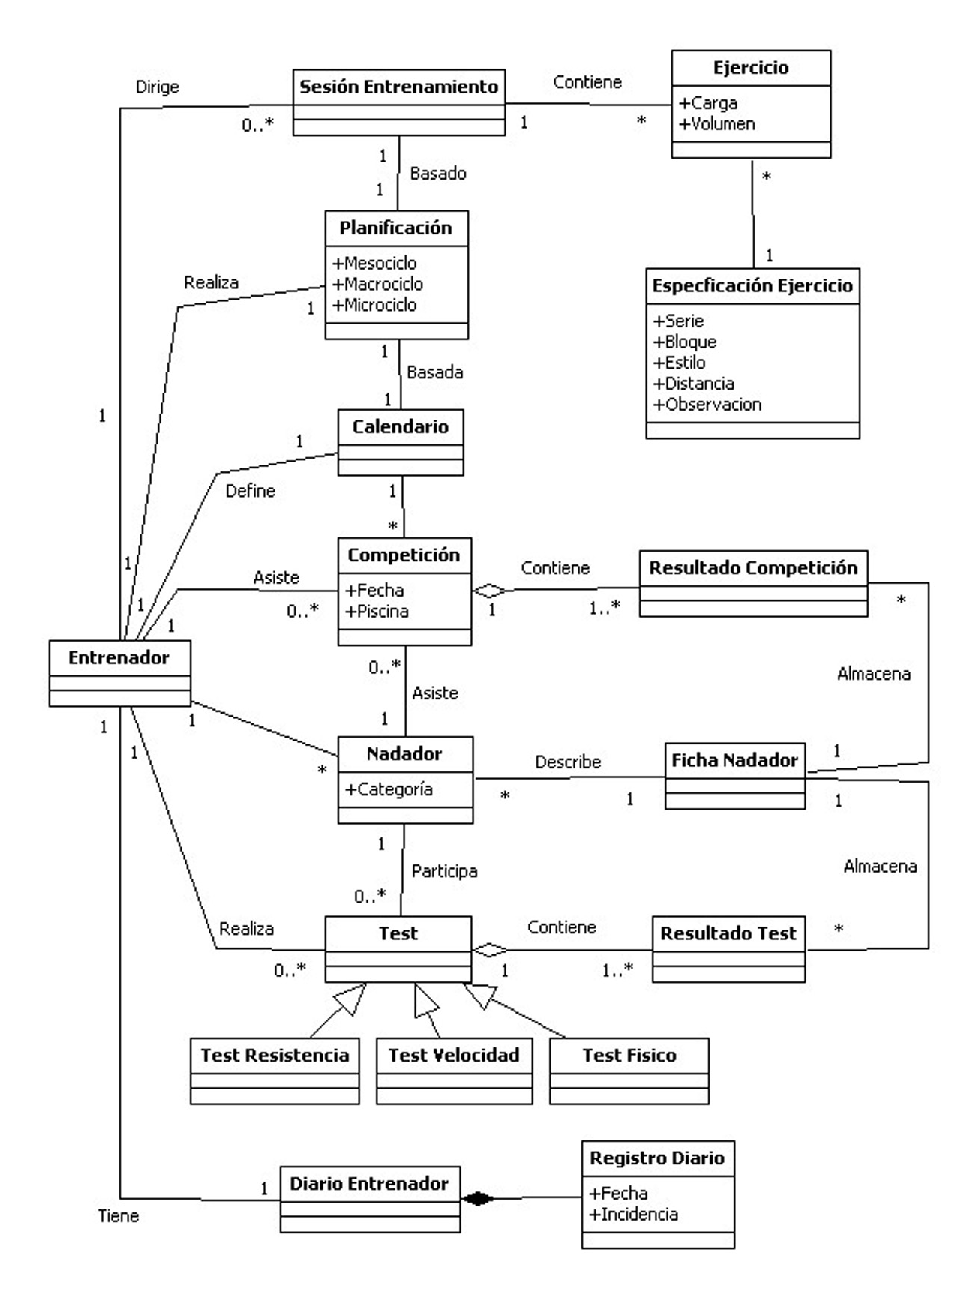
\includegraphics[width=400px]{./eps/captreq_modelo_dominio.eps}
	  \caption{Diagrama del modelo del dominio}
	  \label{fig:modelo_dominio}
	\end{figure}
% subsection construcción_del_modelo_del_dominio (end)

% section modelo_del_dominio (end)

% chapter captura_de_requisitos (end)